O objetivo da pesquisa é caracterizar dimensões afetivas negativas em perfis do twitter localizando pontos comuns entre usúarios portadores de afetividades negativas (stress, ansiedade e depressão) de mesmo nível. Esse tipo de processo se asemelha com a aprendizagem não supervisionada, logo, antes dessa etapa é necessário mapearmos atributos, sendo assim, é necessário a identificação de usúarios com dimensões afetivas negativas em primeiro momento.

Como observado, existem vários passos para conclusão desse projeto, abertamente estrutura de processamento contára com um processo de mineração e dois processos de inteligencia artificial afim de gerar dois modelos lógicos. O primeiro modelo responsavel por inferir valores da EADS em um perfil, e o segundo, de predizer, a partir de dados do perfil, a probabilidade de existir um determinado nível de afetividade utilizando dados do perfil.

O projeto em geral tem alguns outros pontos sociais envolvidos, que assim, tornam a área de atuação da pesquisa um pouco mais ampla, entretando nenhum desses pontos, exceto a utilização de profissionais capacidados para geração de alguns atributos na base da pesquisa, impactam diretamentamente a \textit{performance} e por isso não serão detalhados. Logo essa documentação é voltada unicamente ao sistema que será desenvolvido.

Pode-se observar na Figura \ref{fig:tecnologias}, o sistema é divido em dois núcleos, o Dumont responsável por minerar e gerar toda a base de dados, e o 14BIS que será responsavel pelas Inteligencias Artificias. O aparente terceiro núcleo, na realidade, é simplesmente um banco de dados embutido gerado pelo APPA (ferramenta de administração de mineração de dados) dentro do Dumont e que será consumido pelo 14BIS posteriormente.

\begin{figure}
    \centering
    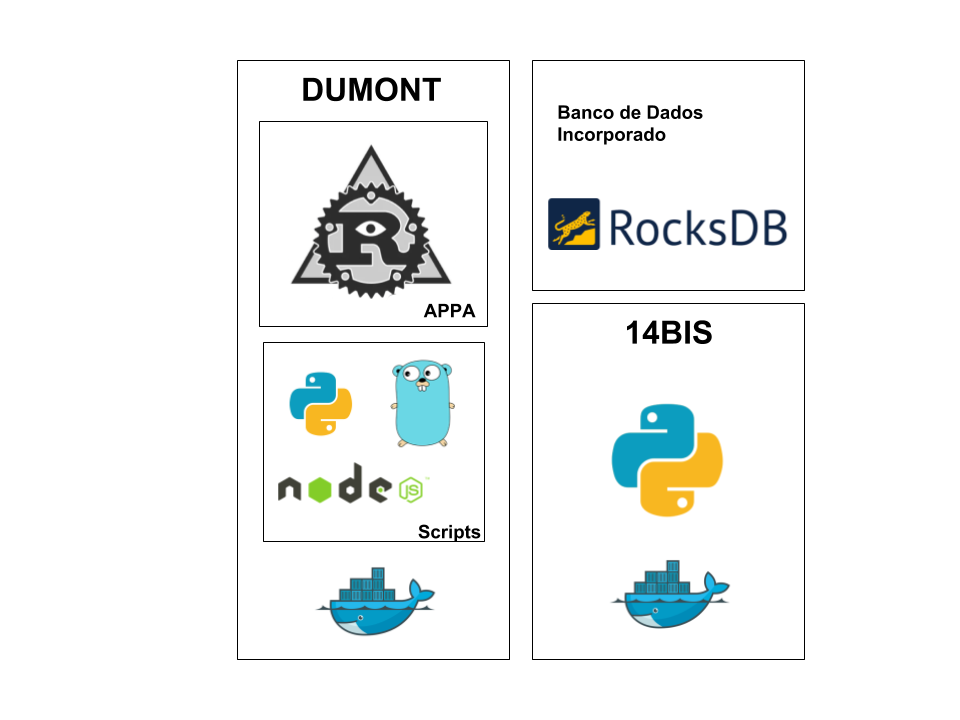
\includegraphics[width=.8\textwidth]{imagens/tecnologias.png}
    \caption{Desenho apresentando os núcleos do projeto}
    \label{fig:tecnologias}
\end{figure}

Existem basicamente 5 técnologias que estão sendo utilizadas nesse projeto:
\begin{itemize}
 \item Rust: Rust é uma linguagem altamente performatica, preza por custo zero em abstração, atua com excelencia em processamento paralelo e seu modelo de alocação de memória evita \textit{dataraces}\footnote{O termo \textit{datarace} traduzido abertamente como corrida de dados é um termo muito utilizado em processamento paralelo e envolve a tentativa de uso de uma alocação de memória por diferentes partes do sistema em um mesmo periodo de tempo}.
 \item Python: É a linguagem atual mais utilizada no mundo de Aprendizado de Máquina, sua simplicidade ja á torna simples de usar, porém, a quantidade de materiais, bibliotecas e artigos sobre PLN e Aprendizado de Máquina á tornam a principal linguagem nesse projeto.
 \item Node/Javascript: Node é o interpretador que permite com que seja possivel executar o Javascript (linguagem originalmente de navegar no servidor). A linguagem tem um grande ganho com integrações e será utilizada para consumir recursos vindos de APIs.
 \item Go: Asemelha-se muito com Rust, porém, tem um ambiente menos burocratico devido a seus diferentes objetivos. Go será a escolha para qualquer processo que não envolva API ou PLN.
 \item RocksDB: O RocksDB é um banco não relacionado, estrutura é baseada em duas \textit{strings} uma sendo chave e a segunda sendo um valor relacionado a essa chave. Bancos não relacionais tendem a ter leitura mais rápida que bancos relacionais, a estrutura do Rocks é baseada em logs e escrito em baixo nivel o que permite sua escrita ser tão rápida quanto sua leitura.
 \item Docker: Docker é uma ferramenta para infra-estrutura, será utilizado para rodar a aplicação em containers e facilitar o \textit{deploy}\footnote{Vindo do termo em inglês "lançar" é utilizado para o ato de colocar uma aplicação em ambiente de produção}.
\end{itemize}

Existirá uma sessão explicando o funcionamento do APPA, e como serão desenvolvidos os scripts que ele ira gerenciar, tanto quanto a parte explicativa sobre a Inteligencia Artificial, logo, nessa introdução os casos de uso serão tratados de forma sucinta. Se observar a Figura \ref{fig:tcc_caso_de_uso}, notara que o Dumont ira utilizar da API do twitter para coletar dados públicos, posteriormente esses dados serão processados e mutacionados a fim de gerar uma base de dados, por final essa base dados será salva em um banco embutido. Tanto o Dumont quanto o 14BIS irão consumir os dados salvos, porém é responsabilidade do 14BIS consumi-los a fim de treinar as IAs desse projeto para gerar os modelos lógicos.

\begin{figure}
    \centering
    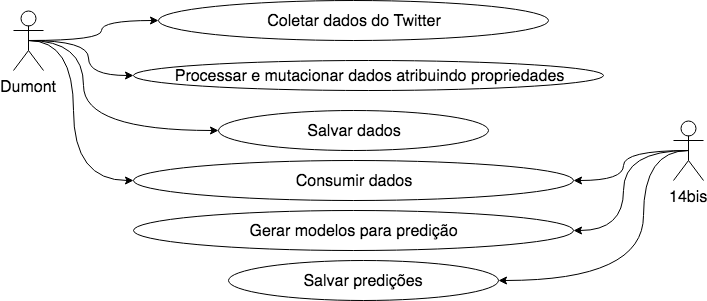
\includegraphics[width=.8\textwidth]{imagens/tcc_caso_de_uso.png}
    \caption{Diagrama de caso de uso do sistema}
    \label{fig:tcc_caso_de_uso}
\end{figure}

Para melhor entendimento a documentação será dividida em núcleos teóricos e práticos. Primeiramente será dado toda a descrição teórica sobre a escolha de atributos, e funcionamento das ferramentas que serão utilizadas no processo. Em seguida será detalhado os núcleos mais práticos como a coleta e mineração, onde alem de explicar como rodar o Dumont, tambem serão explicados como e por que foram construidas essas partes do sistema. Como ja dito, a primeira etapa se consiste em entender alguns dos atributos utilizados aqui.

\section{Engenharia de Atributos}
A escolha dos atributos, também intitulada popularmente como \textit{feature engineering}, é o ato mais importante durante a mineração de dados, por que é através desses atributos que as maquinas irão aprender. É válido destacar que essa sessão serve apenas para introduzir a razão dos atributos, seu detalhamento será dado durante a sua implementação.

O primeiro atributo relevante aqui é o sentimento. Já que será abordado dimensões afetivas negativas, o sentimento expressado por uma frase tem um grande impacto como atributo. Entretanto, o sentido em uma frase pode ser mais fácil de ser extraído em textos concisos, ou seja, normalizar os textos é necessário.

Um dos atributos utilizados aqui será o texto normalizado, para isso será utilizado o \textit{spacy}, uma biblioteca Python para remover palavras que oferecem apenas ruídos ao resultado. Além disso, também será tirada a arvore sintática, para que seja possível estabelecer padrões de discurso na IA, ou então, reconhecer certas palavras presentes em demais analises.

Uma vez observado os nossos atributos, seria necessário erguer um sistema capaz de realizar tarefas e persistir esses dados em algum banco de dados. Porém, será utilizado nessa pesquisa uma ferramenta para gerenciar tais tarefas.

\section{\textit{Application to Process and Produce Analytic Data (APPA)}}

Definir uma boa base de dados é o ponto mais critico durante a criação de uma inteligência supervisionada. O \textit{Application to Process and Produce Analytic Data} (APPA), ou, Aplicação para Processamento e Produção de Dados Analíticos, é um ferramenta criada capaz cadastrar tarefas, em qualquer linguagem e utilizar delas para coletar e processar esses dados afim de gerar uma base de conhecimento.

Explicando com mais detalhes, a figura \ref{fig:appa_eng} mostra o funcionamento da ferramenta. Existe uma arquivo chamado \textit{config.yml} que tem mapeado todas as tarefas e entidades de processamento. Essas tarefas podem ser escritas em qualquer linguagem de programação e algumas delas podem ser responsáveis por coletar dados, os scripts que são escritos com intuito de retornar dados para processamento são chamados coletores.

\begin{figure}
    \centering
    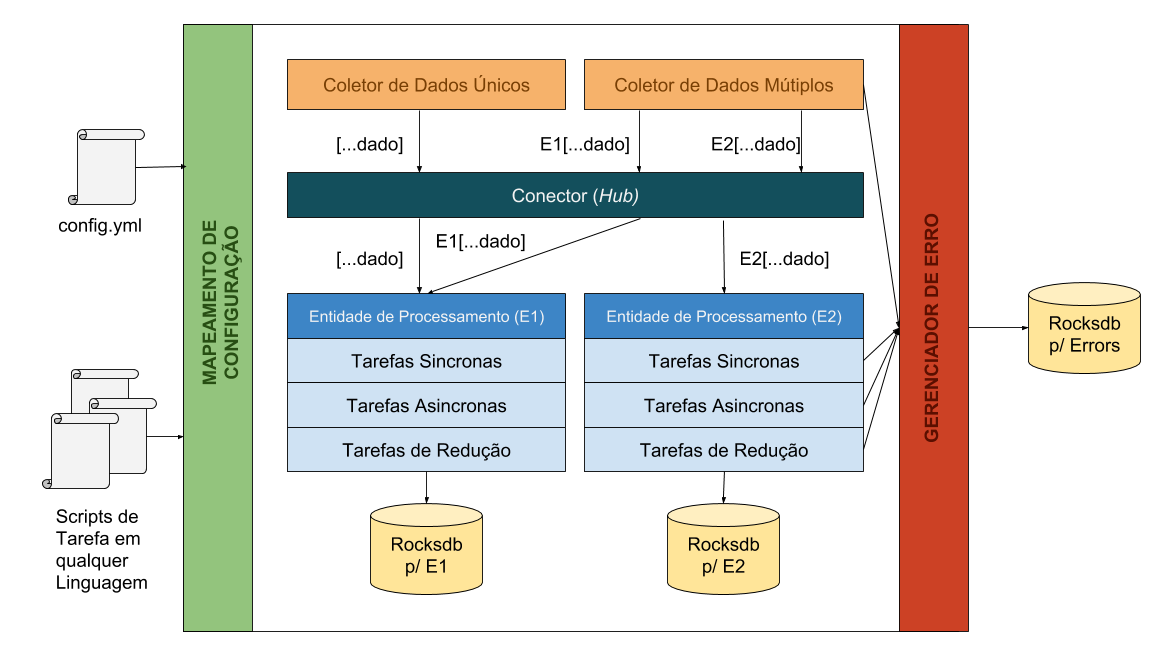
\includegraphics[width=.8\textwidth]{imagens/appa_eng.png}
    \caption{Diagrama demonstrando o funcionamento da ferramenta APPA}
    \label{fig:appa_eng}
\end{figure}

Um dado emitido por um coletor é marcado ou não por uma \textit{tag}, ou marcação, essa responsável por creditar qual coletor será responsável por processar. Por padrão um dado enviado sem destino é marcado com o simbolo \textit{underline}. Toda tarefa dentro do APPA é considerada uma tarefa com múltiplas saídas, logo, é possível enviar dados em lotes e tempo real para que o APPA processe dentro das entidades. 

Entidades de processamento, por sua vez, são compostas por coletores e tarefas de processamento. As tarefas de processamento podem ser síncronas ou assíncronas, ambas executam individualmente por unidade de dado, algo similar a uma linha de dados de um banco, a diferença é seu formato de execução, como o próprio nome fala as tarefas assíncronas não respeitam ordem de execução e são executadas paralelamente pelo processador. Alem disso existem as redutoras e/ou mapeadoras, consumiram todo o banco gerado após a execução das tarefas síncronas e assíncronas e retornara um novo estado para o banco total. Cada entidade gera seus dados em um banco incorporado isolado para os dados processados por elas.

Diferente de outras ferramentas, o processo de mineração nunca é interrompido. Qualquer erro que aconteça na aplicação é gerenciado por uma camada e registrado em um banco de erros, após isso o processamento segue para os demais dados.

\section{Tarefas de Processamento}
Como explicado, o APPA ira gerenciar nossas tarefas de processamento, ja foi abordado também alguns atributos que serão necessários para 14BIS executar os modelos lógicos. Tendo isso em vista é necessário que seja implementado \textit{scripts} de mineração e pré-processamento para que a base de dados de dados do projeto tenha a estrutura necessária para que as IAs possam agir.

Essa sessão tem como objetivo detalhar os atributos e \textit{scripts} criados para gerar-los. Além disso em alguns casos, onde são utilizados recursos externos como APIs, será detalhado a configuração necessária.

É importante ressaltar que todo o projeto é \textit{Open Source}, conhecidos como projeto de código aberto, e todo o código criado para esse projeto pode ser encontrado na plataforma de versionamento do GitHub\footnote{\url{https://github.com/getdumont}}.

Antes de iniciarmos as explicações é necessário que para reprodução dessa pesquisa você tenha inicialmente o Docker\footnote{\url{https://www.docker.com/}} instalado. Caso deseje executar as tarefas individualmente, como será citado aqui, é necessário que você tenha instalado na sua máquina o Python 3.6\footnote{\url{https://www.python.org/downloads/release/python-360/}} e o NodeJS 9.11\footnote{\url{https://nodejs.org/en/blog/release/v9.11.1/}}. Vale lembrar que todo código aqui demonstrado foi escrito, executado e testado em um sistema operacional com base Unix, logo a portabilidade com Windows não é garantida.

Uma vez com as ferramentas instaladas no sistema operacional, torna-se possível a reprodução dessa pesquisa. A primeira etapa como já discursada até então se refere a coleta de dados.

\subsection{Tarefa de Coleta}
A coleta será feita utilizando a API publica do twitter, o link para a documentação é \url{https://developer.twitter.com/en/docs}. Será trabalhado no projeto duas entidades: Tweet e Usuário. O tweet é a entidade que representa a publicação do usuário, enquanto o usuário contém informações necessárias sobre o seu perfil.

Para que seja possível acessar a API é necessário criar uma conta de desenvolvimento e gerar o \textit{token} de acesso\footnote{\url{https://apps.twitter.com/app/new}}. Com a chave em mãos é possível replicar o arquivo /collector/client/.env\_sample dentro do projeto Dumont para /collector/client/.env, e conforme demonstrado na figura \ref{fig:twitteropts}, completar os campos necessários.

Para rodar basta executar o comando \textit{node collector/twitter.js}, e verá a saída de dados. Existem duas observações relevantes a serem feitas nessa etapa:
\begin{itemize}
  \item !AppaTag(tweet) e !AppaTag(user): Se notar, algumas linhas começarão com essas duas anotações, são essas anotações que serão responsáveis por fazer com que o APPA identifique qual entidade de processamento será responsável por processar cada tipo de dado.
  \item Dados de Emoji: É possível notar que alguns dados mapeados não existem na API do Twitter. Como observado, um dos problemas durante a mineração de dados é o uso de \textit{emojis} em textos, já citado também, é possível algumas tarefas de pré-processamento serem executadas durante a própria coleta. Sabendo que emojis podem expressar sentimentos \cite{novak2015sentiment}, e que armazenar e tratar esse dado poderia ser relevante na hora de confirmar sentimento em frases, o autor também criou a biblioteca \textit{Emojinator}\footnote{https://github.com/getdumont/emojinator}, além do texto tradado, também será obtida informações do \textit{emojis} utilizados no meio do texto.
\end{itemize}

\begin{figure}
    \centering
    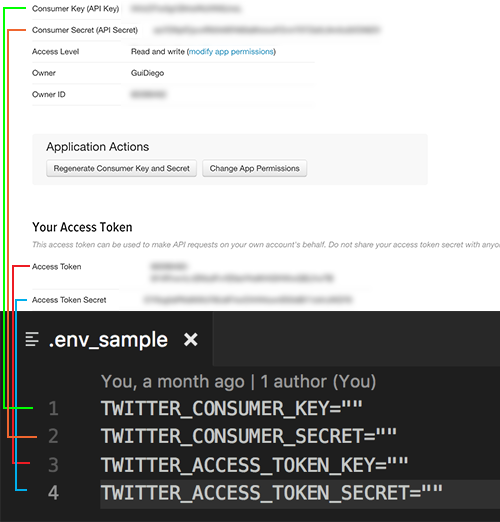
\includegraphics[width=.8\textwidth]{imagens/twitteropts.png}
    \caption{Imagem demonstrando onde cada chave deve ser inserida no código}
    \label{fig:twitteropts}
\end{figure}

Uma vez configurado o coletor, ainda é necessário entender e configurar as outras tarefas para que o APPA funcione apropriadamente, logo, é necessário entender como essas entidades ficarão no final e quais as tarefas que realizarão essa manipulação.

